\section{Introduction}

Geometric algorithms are often difficult to implement and convey to others.
Algorithm \emph{implementers} must correct programming errors and handle
degenerate situations correctly. Traditional debuggers provide only textual or
numerical representations of geometric data structures, and generating
degenerate geometric input is a nontrivial task for which there is often little
assistance. Algorithm \emph{presenters} must convey their ideas to audiences of
researchers and students. Many presenters use static depictions and verbally
explain algorithm mechanics, a type of presentation that does not fully capture
the dynamic nature of geometric algorithms.

A \emph{geometric workbench} aids algorithm implementers and presenters by
providing facilities to dynamically visualize geometric algorithms. Implementers
can visually inspect geometric relationships and properties of data structures,
quickly recognizing erroneous computations. Presenters can produce
animations of their algorithms, more clearly conveying essential
ideas to their audience. Both types of geometers can interactively control the
flow of execution and easily generate degenerate input data.

\begin{figure}[h]
	\centering
	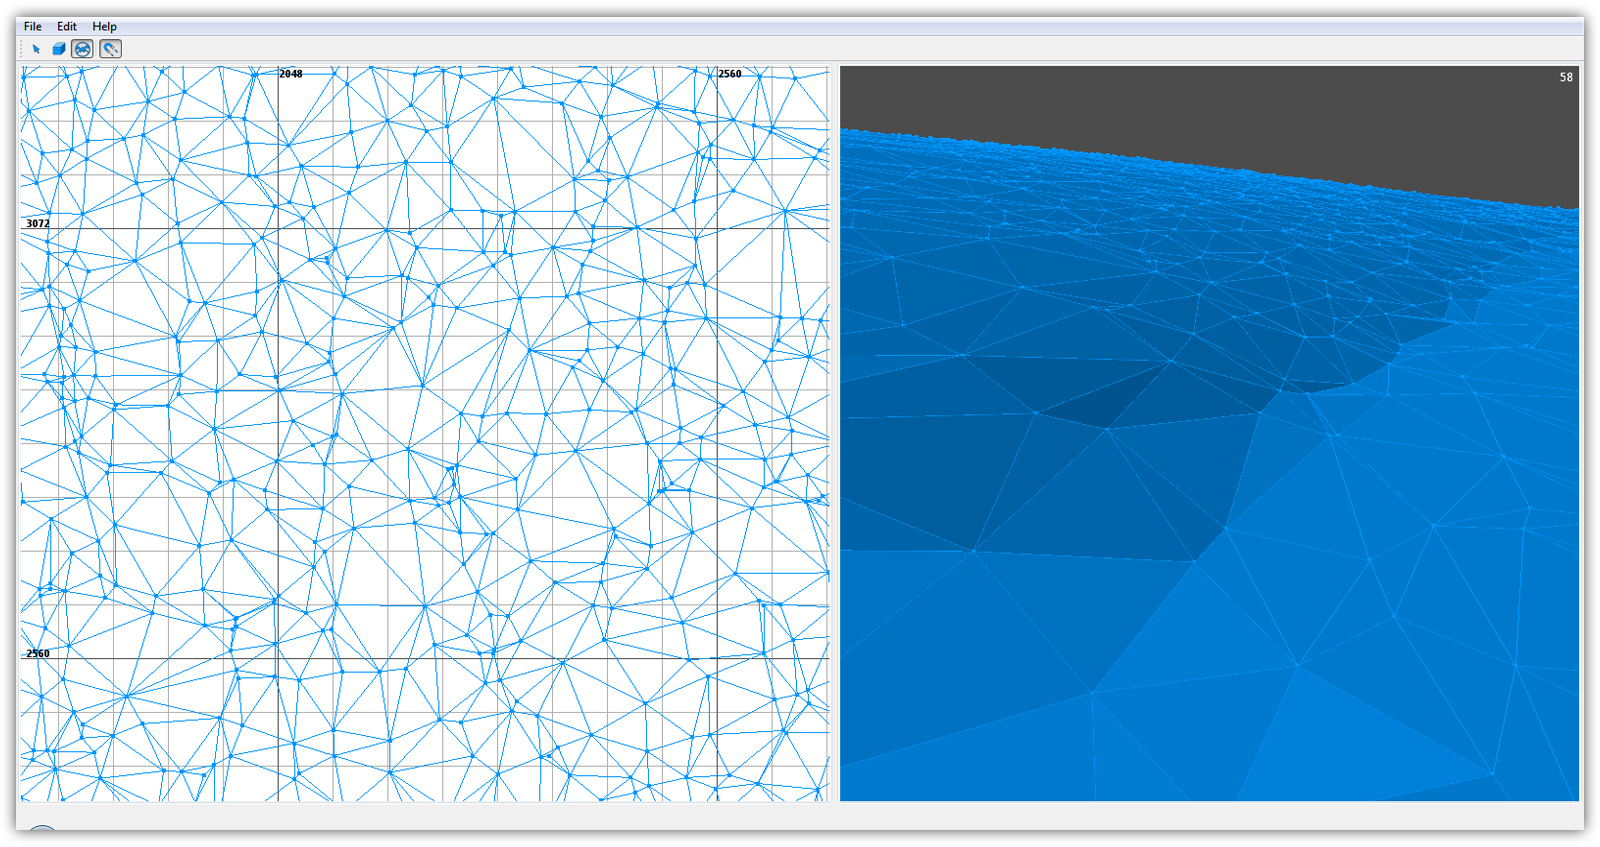
\includegraphics[width=\textwidth]{figures/currentstate-2}
	\caption{Our workbench animates incremental terrain mesh generation.}
	\label{fig:currentstate}
\end{figure}

\emph{Degree-driven algorithm design} encourages robust geometric computing by
attempting to minimize an algorithm's arithmetic precision with its running time
and space~\cite{millman2012degree}. Millman built a C++ library (DDAD) to
facilitate implementing algorithms with low degree predicates. Our workbench
extends DDAD with a visual event system and provides a standalone GUI that can
generate input data and render algorithm execution.
Figure~\ref{fig:currentstate} captures the workbench rendering a terrain mesh
built by incremental delaunay triangulation.

[todo: paragraph overviewing the paper]

% Section 2 reviews previous work. Section 3 recalls a general framework for
% designing software visualization systems. Section 4 uses the framework to
% explain our workbench desiderata. Section 5 provides an architectural overview
% of the workbench and section 6 runs through a case study of animating a convex
% hull algorithm. Section 7 concludes by explaining how current workbench
% architecture supports our desiderata and identifies areas in which it can
% improve.